\section{結果および考察}
\subsection{近接2粒子ホログラムの検証実験}
Table \ref{table:stripePatternExperiment}に示した条件で記録したホログラムと,そのフーリエ変換で得たスペクトル分布の例を Fig. \ref{fig:stripePatternExpExample} に示す.Fig. \ref{fig:stripePatternExpExample:a}は撮影したホログラムであり,Fig. \ref{fig:stripePatternExpExample:b}は中央のホログラムフリンジパターンをクロップした画像である.この画像に対して二次元フーリエ変換と対数変換,正規化を施したスペクトル分布画像を Fig. \ref{fig:stripePatternExpExample:c} に示す.Fig. \ref{fig:stripePatternExpExample:c} において,画像中央の低周波数域に粒子近接に伴う縞パターンが現れていることが確認できる.Fig. \ref{fig:2particleSpectrum}に示すように縞パターンは周波数域全域に現れるが,実験データでは背景ノイズなどの高周波成分で高周波数域では縞パターンが確認できなくなる.

$y$軸方向の粒子間距離 $\Delta \eta$ は常に0であることに注意して,記録したスペクトル分布画像から粒子間距離 $\Delta \xi$ を算出する.$1 \leq x \leq 512$,$247 \leq y \leq 266$領域のスペクトルを,$y$軸方向に縮約して得る$x$軸方向の512次元ベクトルをフーリエ変換して得るスペクトルを Fig. \ref{fig:stripePatternFourierSignal}に示す.この図では,Fig. \ref{fig:stripePatternExpExample}に示す粒子間距離 $\Delta \xi = \SI{320}{\um}$のデータに対するスペクトルを示している.このプロットでは,$x=0$で分布のバイアスのピークが立ち,その次の最大値として縞パターンを示すピークが立っている.このピークの位置を検出することで,粒子間距離 $\Delta \xi$ を推定することができる.この例では,灰色の線で示す,記録条件から算出される縞パターンのピーク位置と推定結果が一致していることがわかる.

以上の手続きで,すべての記録ホログラムに対して粒子間距離を推定した結果を Fig. \ref{fig:stripePatternDetection}に示す.横軸は実験で設定した粒子間距離 $\Delta \xi$ を粒子径$2a$で除した値であり,縦軸は推定された粒子間距離のピクセルベースの値 $l\, \si{[pixel]}$ である.このプロットでは,粒子間距離が2つの粒子半径の和より大きい,すなわち2つの粒子が重複しない限りでは,推定された粒子間距離が実験で設定した粒子間距離とよく一致していることがわかる.一方で,2つの粒子が重複する場合はピーク検出精度が低下する.これは,式(\ref{th:extratermsApprox})に示す近似式が,2つの粒子が重複する場合には成立しないためである.

以上から,奥行方向距離を持たない同径粒子が重複しない条件で,式(\ref{th:2particleSpectrum})に示すスペクトル分布パターンと式(\ref{th:stripepattern})に示す縞パターンの推定方法が有効であることを確認した.

\begin{figure}[H]
    \centering
    \begin{subfigure}[c]{0.45\linewidth}
        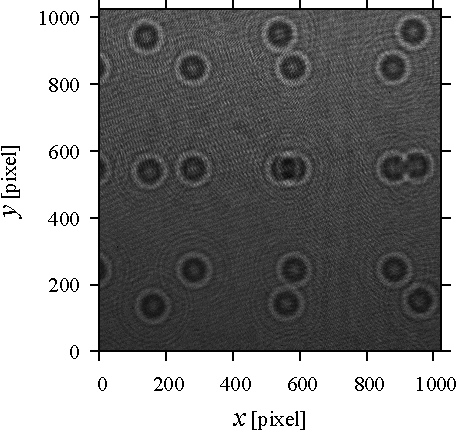
\includegraphics[width=\linewidth]{./Figure/4_Results/stripe_pattern_experiment/recorded_data/a.pdf}
        \caption{Recorded hologram image}
        \label{fig:stripePatternExpExample:a}
    \end{subfigure}
    \hfill
    \begin{subfigure}[c]{0.45\linewidth}
        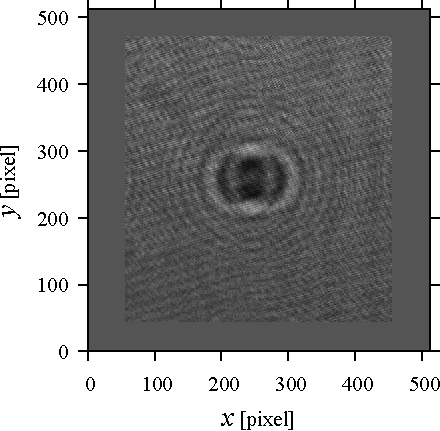
\includegraphics[width=\linewidth]{./Figure/4_Results/stripe_pattern_experiment/recorded_data/b.pdf}
        \caption{Cropped hologram image of Fig. \ref{fig:stripePatternExpExample:a}}
        \label{fig:stripePatternExpExample:b}
    \end{subfigure}

    \begin{subfigure}[b]{0.8\linewidth}
        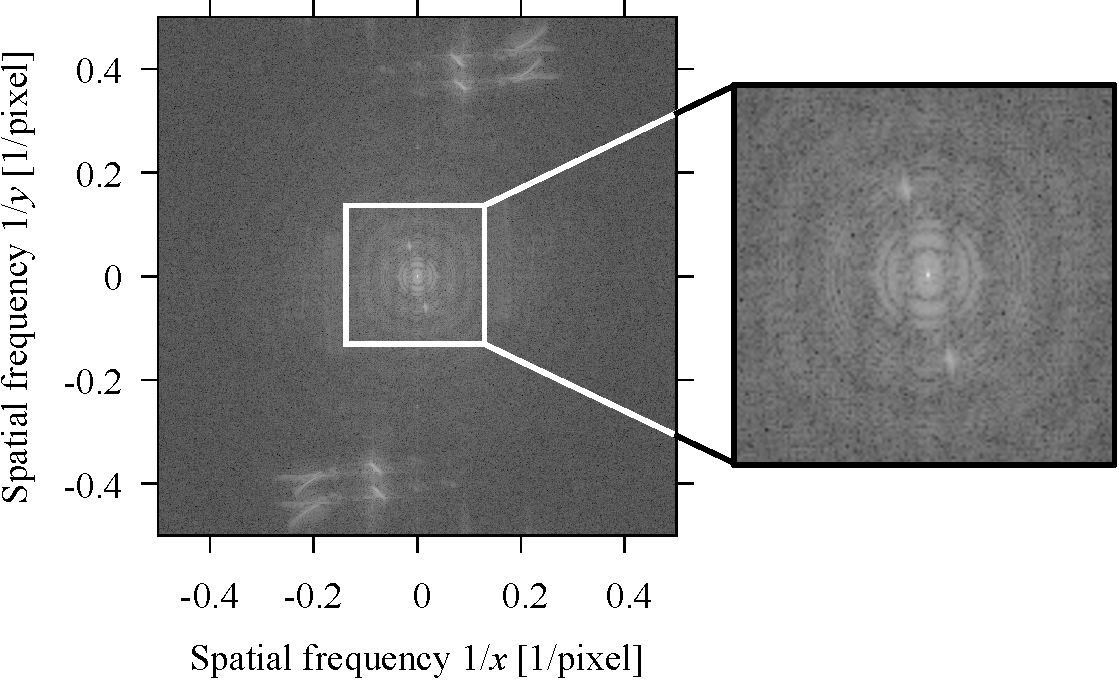
\includegraphics[width=\linewidth]{./Figure/4_Results/stripe_pattern_experiment/recorded_data/c.pdf}
        \caption{Computationally calculated spectrum of the hologram Fig. \ref{fig:stripePatternExpExample:b}}
        \label{fig:stripePatternExpExample:c}
    \end{subfigure}

    \caption{Example of a hologram and its spectrum. Here, the horizontal particle distance $\Delta \xi$ is \SI{320}{\um}.} 
    \label{fig:stripePatternExpExample}
\end{figure}

\begin{figure}[H]
    \centering
    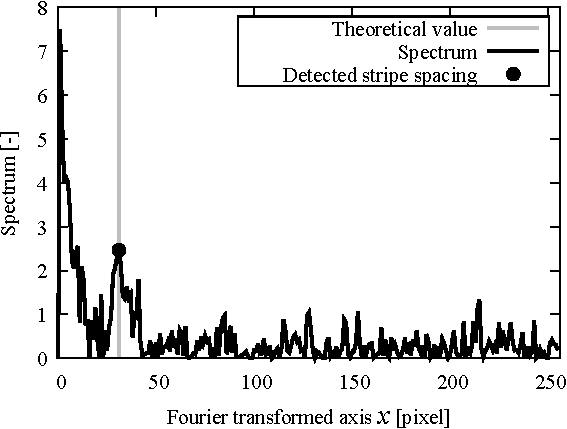
\includegraphics[width=0.75\linewidth]{./Figure/4_Results/stripe_pattern_experiment/stripe_pattern_exp_exam_peak.pdf}
    \caption{Fourier-transformed signal of the shrunk spectrum vector. A peak due to vector bias exists at $x=0$, and a peak representing the stripe pattern can be seen as the next maximum value. The gray line indicates the theoretical value of the stripe pattern peak position.}
    \label{fig:stripePatternFourierSignal}
\end{figure}

\begin{figure}[H]
    \centering
    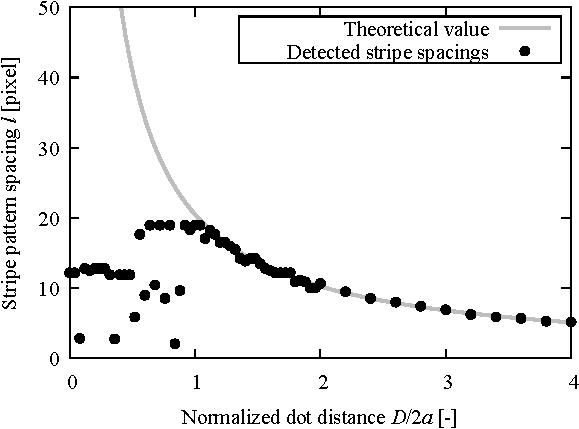
\includegraphics[width=0.75\linewidth]{./Figure/4_Results/stripe_pattern_experiment/stripe_pattern_exp_final_result.pdf}
    \caption{Detected particle distance $l\, \si{[pixel]}$ for each particle distance $\Delta \xi / 2a$. The horizontal axis is the particle distance $\Delta \xi$ normalized by the particle diameter $2a$. The detected peak agrees well with the theoretical value if the two particle do not overlap.}
    \label{fig:stripePatternDetection}
\end{figure}



\subsection{水滴近接検出モデルの性能評価および実験データに対する推論}\label{sec:modelEvalResult}
近接水滴ホログラムを抽出するためのEfficientNetV2-SおよびEfficientNetV2-XLモデルを\ref{sec:EffNetV2}節で定義した.生成したデータで学習したモデルの性能評価と,実験データに対する推論結果を示す.式(\ref{th:2particleSpectrum})ではホログラムをフーリエ変換して得たスペクトル分布に対する縞パターン抽出を行ったが,フーリエ変換は可逆変換であるため,ホログラムをそのまま入力としてモデルに学習させることも原理的に可能である.ホログラムをフーリエ変換せず直接学習できる場合,ホログラムの前処理にかかる計算時間を削減できる.そこで,まずホログラムをそのまま入力として学習したモデルと,フーリエ変換を施したホログラムを入力として学習したEfficientNetV2-Sモデルの2つを比較する.前処理としてフーリエ変換を行うモデルの学習曲線をFig. \ref{fig:fftmodel}に,フーリエ変換を行わずホログラムから直接学習するモデルの学習曲線をFig. \ref{fig:rawmodelS}に示す.学習曲線は,学習の進行をあらわす単位であるepochに対する損失関数値やAccuracyのプロットである.1 epoch は学習データに用いるすべてのデータが一度モデルに入力されパラメータ更新される単位をあらわす.いずれのモデルでも,損失関数値・Accuracyともに同等の値まで向上し収束していることがわかる.また,学習していないデータによる検証結果をあらわすvalidation loss・validation Accuracyも,学習データに対する損失関数値・Accuracyと同等の値まで向上している.これらの結果から,ホログラムをフーリエ変換して得たスペクトル分布を入力として学習したモデルと,ホログラムをそのまま入力として学習したモデルの性能は同等であり,過学習を起こさずに学習できていることがわかる.したがって,本論文では,実験データに対する衝突抽出のために,数値生成ホログラムをフーリエ変換せず直接学習したEfficientNetV2-XLを用いる.

EfficientNetV2-XLモデルの学習曲線をFig. \ref{fig:rawmodelXL}に示す.このモデルの学習には1 epochあたり約6時間ほどかかる.時間制約のため22 epochで学習を打ち切っている.EfficientNetV2-Sモデルでは学習データに対するAccuracyの最大値は0.846であったが,EfficientNetV2-XLモデルでは0.853となり,モデルの性能が向上していることがわかる.EfficientNetV2-XLモデルの検証データに対する損失値やAccuracyから,このモデルは過学習を起こさずに学習できていることを確認できる.しかし,検証データに対する学習曲線はEfficientNetV2-Sモデルほど学習データの曲線に追従しておらず,EfficientNetV2-SモデルのAccuracyよりも低い値である.したがって,以降ではEfficientNetV2-SとEfficientNetV2-XLモデルそれぞれに対して,数値生成ホログラムに対する近接検出性能を評価する.

\begin{figure}[H]
    \centering
    \begin{subfigure}[t]{0.45\linewidth}
        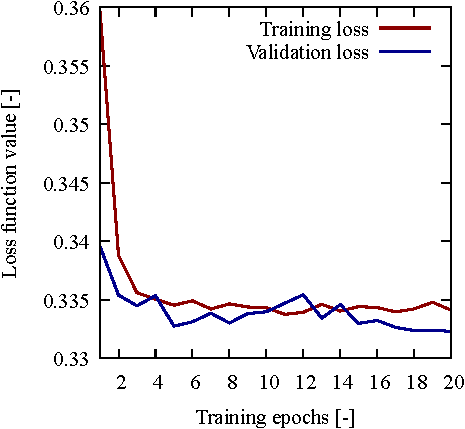
\includegraphics[width=\linewidth]{./Figure/4_Results/training/loss_fft.pdf}
        \caption{Loss improvement of the FFT-preprocessed model}
        \label{fig:fftmodel:loss}
    \end{subfigure}
    \hfill
    \begin{subfigure}[t]{0.45\linewidth}
        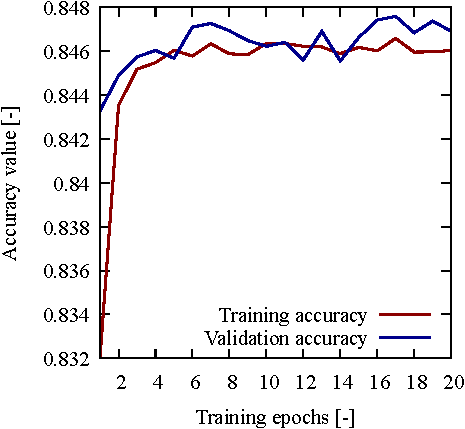
\includegraphics[width=\linewidth]{./Figure/4_Results/training/acc_fft.pdf}
        \caption{Accuracy improvement of the FFT-preprocessed model}
        \label{fig:fftmodel:acc}
    \end{subfigure}

    \caption{Training results of the FFT-preprocessed EfficientNetV2-S model; the model was trained with the dataset of the FFT-preprocessed holograms. The stripe patterns of the proximity droplet holograms were enhanced by the FFT preprocessing, and they can be seen on the center of the spectrum. Detailed model architecture is shown in Table \ref{table:EffNetV2-S}.} 
    \label{fig:fftmodel}
\end{figure}

\begin{figure}[H]
    \centering
    \begin{subfigure}[t]{0.45\linewidth}
        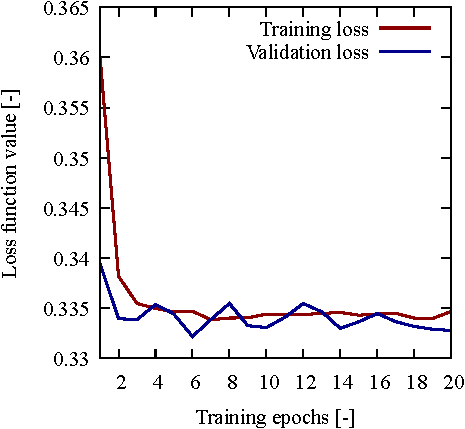
\includegraphics[width=\linewidth]{./Figure/4_Results/training/loss_raw.pdf}
        \caption{Loss improvement of the raw-input model}
        \label{fig:rawmodelS:loss}
    \end{subfigure}
    \hfill
    \begin{subfigure}[t]{0.45\linewidth}
        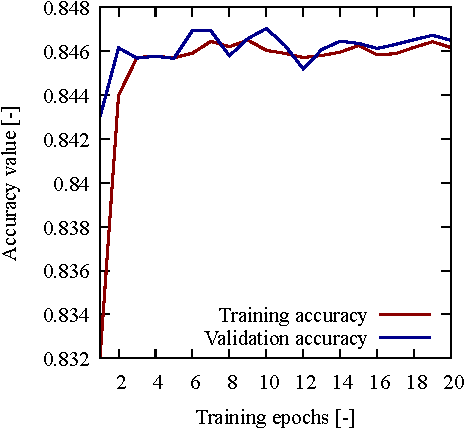
\includegraphics[width=\linewidth]{./Figure/4_Results/training/acc_raw.pdf}
        \caption{Accuracy improvement of the raw-input model}
        \label{fig:rawmodelS:acc}
    \end{subfigure}

    \caption{Training results of the raw-input EfficientNetV2-S model; the model was trained with the dataset of the raw holograms. The model can detect the proximity droplets without the FFT preprocessing because Fourier transform is a reversible operation. Detailed model architecture is shown in Table \ref{table:EffNetV2-S}.} 
    \label{fig:rawmodelS}
\end{figure}

\begin{figure}[H]
    \centering
    \begin{subfigure}[t]{0.45\linewidth}
        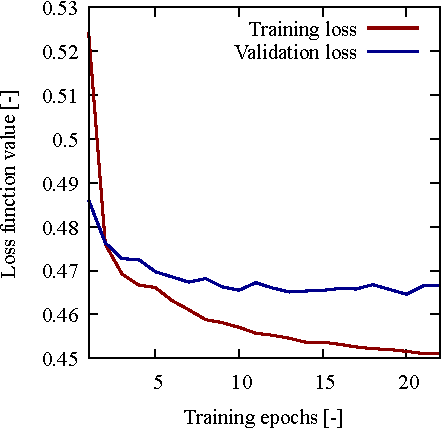
\includegraphics[width=\linewidth]{./Figure/4_Results/training/lossXL.pdf}
        \caption{Loss improvement}
        \label{fig:rawmodelXL:loss}
    \end{subfigure}
    \hfill
    \begin{subfigure}[t]{0.45\linewidth}
        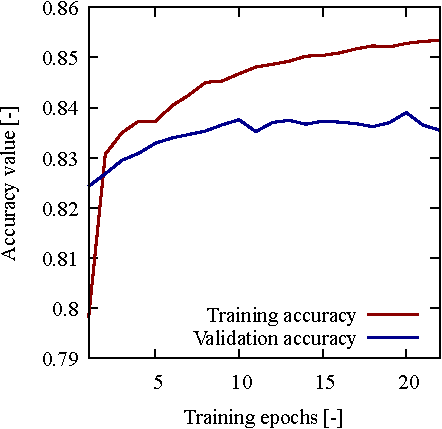
\includegraphics[width=\linewidth]{./Figure/4_Results/training/accXL.pdf}
        \caption{Accuracy improvement}
        \label{fig:rawmodelXL:acc}
    \end{subfigure}

    \caption{Training results of the raw-input EfficientNetV2-XL model; the model was trained with the dataset of the raw holograms. Detailed model architecture is shown in Table \ref{table:EffNetV2-XL}.} 
    \label{fig:rawmodelXL}
\end{figure}


数値生成したホログラムデータで学習したEfficientNetV2-SおよびXLモデルに対して,数値生成した10000枚のホログラムを用いて近接検出性能を統計的に評価する.学習に用いたデータの画像サイズは$256\times 256 \,\si{pixel^2}$だが,ここで性能評価に用いるデータは$1024 \times 1024 \,\si{pixel^2}$のものであり,実験によって得られるデータを模擬している.すなわち,モデルは入力データを$x$軸$y$軸それぞれ4分割した計16個の領域に対して推論を行い,それらの領域に対する近接粒子の存在確率を0から1の値で示す.数値生成データに対する推論の可視化結果の例をFig. \ref{fig:numericalInfResult}に示す.近接粒子の存在確率は各領域に重畳した赤色のシェードの濃淡であらわす.また,真の近接粒子の重心座標を緑色の十字印で示す.この例では,EfficientNetV2-S/XLともに十分高い確率で正しい領域の粒子近接確率を出力しているが,近接粒子と関係のない領域も高い値で予測していることがわかる.この例でも確認できるそれぞれのモデルによる推論の傾向として,EfficientNetV2-XLはEfficientNetV2-Sに比べて偽陽性(FP)が高い確率で出力され,また真陰性(TN)が低い確率で出力される.つまり,EfficientNetV2-XLはEfficientNetV2-Sに比べて,近接粒子が存在しない領域の出力の分散が大きい.このことをTable \ref{table:stddev}に示す.

\begin{table}[H]
    \centering
    \caption{Standard deviation of the inference result of the trained models. The value is calculated from all of numerically generated holograms. The standard deviation of the EfficientNetV2-XL model is larger than that of the EfficientNetV2-S model.}
    \begin{tabular}{cc}
        Model name & Standard deviation \\ \hline \hline
        EfficientNetV2-S & 0.251 \\ \hline
        EfficientNetV2-XL & 0.397 \\
    \end{tabular}
    \label{table:stddev}
\end{table}

\begin{figure}[H]
    \centering
    \begin{subfigure}[t]{0.85\linewidth}
        \centering
        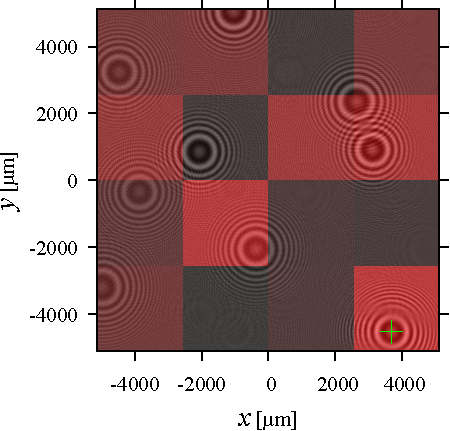
\includegraphics[width=0.7\linewidth]{./Figure/4_Results/training/outholoS.pdf}
        \caption{EfficientNetV2-S model; the model output value at the area including the proximity droplets is \num{1.00}. }
        \label{fig:numericalInfResult:s}
    \end{subfigure}
    \\
    \begin{subfigure}[t]{0.85\linewidth}
        \centering
        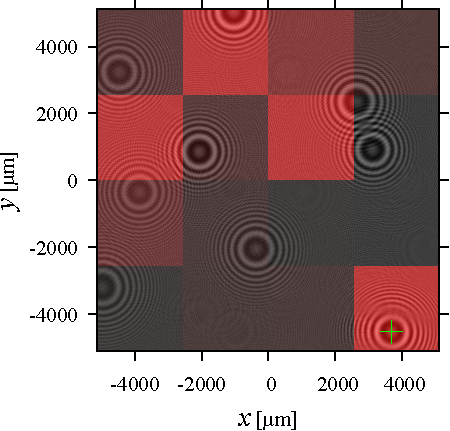
\includegraphics[width=0.7\linewidth]{./Figure/4_Results/training/outholoXL.pdf}
        \caption{EfficientNetV2-XL model; the model output value at the area including the proximity droplets is \num{0.98}. }
        \label{fig:numericalInfResult:xl}
    \end{subfigure}

    \caption{Example of the inference result of the EfficientNetV2-S/XL raw-input model. The proximity droplets are indicated by the green cross symbol. The shade of red overlay indicates the confidence of the model. This output image is contrast-enhanced for visualization.} 
    \label{fig:numericalInfResult}
\end{figure}

また,推論結果の評価指標として,数値生成データに対するAccuracy,Precision,Recallを計算する.これらの定義は\ref{sec:modelEvaluation}節で示した.これらの値は,モデルの出力である近接粒子の存在確率に対する近接判定のしきい値によって変化する.しきい値が0から1までの値に対するこれらの指標のプロットをFigs. \ref{fig:accuracyResult}〜\ref{fig:recallResult}に示す.

Accuracyはいずれのモデルでもしきい値が大きくなると高い値を示す傾向にある.しかし,ここで用いた数値生成データは推論を行った$256 \times 256 \,\si{pixel^2}$の画像のうち15/16,すなわち93.75\%が非近接条件データであるため,仮にモデルがすべてのデータをNegative判定するとAccuracyは93.75\%となる.したがって,Accuracyはこのような不均衡データの場合,有効な評価指標であるとは言えない.

PrecisionはPositiveデータの的中率であり,EfficientNetV2-SがEfficientNetV2-XLに比べて高い値を取っている.Precisionが高い値を取ると,抽出されたデータのうち多くの割合が正しいPositiveデータを含むことになり,その後の手動の確認が容易になる.Table \ref{table:stddev}に示すように,EfficientNetV2-XLはEfficientNetV2-Sに比べて,近接粒子が存在しない領域の出力の分散が大きいため,特にしきい値が大きいときにPrecisionが低い値を取っていることがわかる.

RecallはPositiveデータを取りこぼしなく検出できているかをあらわす指標であり,真にPositiveなデータのうち実際にPositive判定できたデータの割合をあらわす.判定のしきい値が大きくなるとPositive判定のハードルが高くなるため,Recallは小さくなる.いずれのモデルもこの傾向を示している.RecallはPrecisionとトレードオフの関係にあり\cite{saito2015},Precisionが低いときRecallは高い値を示す.本研究の最終的な目的は,水滴の衝突に関わる統計量を正確に得ることであるため,PrecisionよりもRecallの値が高いことが望ましい.その点で,EfficientNetV2-XLはEfficientNetV2-Sに比べて望ましい性能を有していると言える.

同じしきい値に対するPrecision,Recallの値をPrecision-Recall図中の点として取って得たPrecision-Recall曲線をFig. \ref{fig:prcurve}に示す.ゼロ除算によって値を得られていないしきい値が1.0のときのPrecisionについては1.0としてプロットしている.PR-AUCは,PR曲線とPrecision軸,Recall軸が囲む面積で定義され,1に近づくほど不均衡データに対する総合的な性能が高いモデルとして評価される\cite{saito2015}.それぞれのモデルに対するPR-AUCをTable \ref{table:prauc}に示す.EfficientNetV2-XLはEfficientNetV2-Sに比べてPR-AUCが高い値を示しており,不均衡データに対する総合的な性能が高いと言える.

以上の結果から,本論文で構築したEfficientNetV2-S/XLモデルによって個別の近接粒子を抽出可能であることが明らかになった.しかし,水滴衝突に係る統計量を正確に得るためにはRecallが1に限りなく近い値を示す必要があり,さらに,推論結果をユーザが確認するコストを減らすためにPrecisionが可能な限り高い値を示す必要があるため,ここで評価したEfficientNetV2-S/XLモデルは未だ十分な精度を有しているとは言えない.水滴ホログラムに対する近接検出は,画像に対する2値分類問題であり,さらにその分類可能性は\ref{sec:twoParticleHologramFeature}節で示したとおりであるから,推論精度向上のボトルネックとなっているのは学習データあるいは学習手法である.数値生成したホログラムを用いた転移学習では,\ref{sec:EffNetV2}節で示した通り画像認識モデルの一般的な学習手法として最適化手法のAdamと学習スケジューリング手法のStepLRを組み合わせて用いたが,より高精度なRAdam\cite{liu2020}や,EfficientNetV2の原著論文で用いられたRMSProp\cite{yamashita2018},Cosine annealing\cite{loshchilov2017}を用いるなどして学習手法を改善できる可能性がある.

\begin{figure}[H]
    \centering
    \begin{subfigure}[t]{0.45\linewidth}
        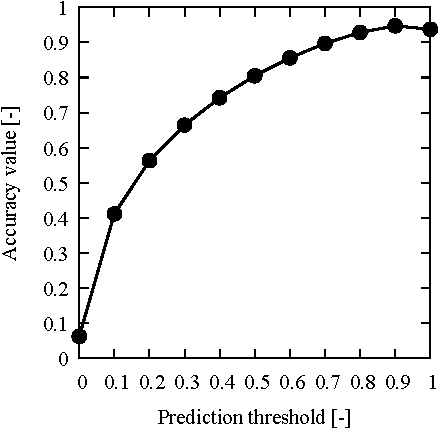
\includegraphics[width=\linewidth]{./Figure/4_Results/training/sresult/acc.pdf}
        \caption{EfficientNetV2-S}
        \label{fig:accuracyResult:s}
    \end{subfigure}
    \hfill
    \begin{subfigure}[t]{0.45\linewidth}
        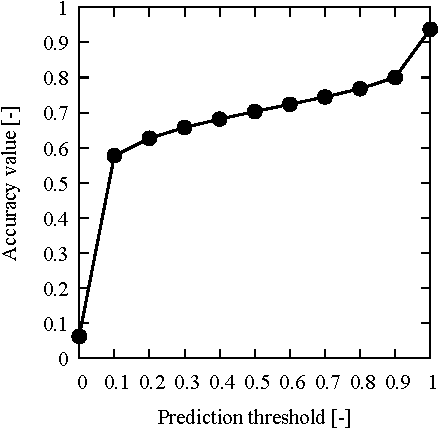
\includegraphics[width=\linewidth]{./Figure/4_Results/training/xlresult/acc.pdf}
        \caption{EfficientNetV2-XL}
        \label{fig:accuracyResult:xl}
    \end{subfigure}

    \caption{Accuracy value for each threshold. The threshold of \num{0.5} is the default value.} 
    \label{fig:accuracyResult}
\end{figure}

\begin{figure}[H]
    \centering
    \begin{subfigure}[t]{0.45\linewidth}
        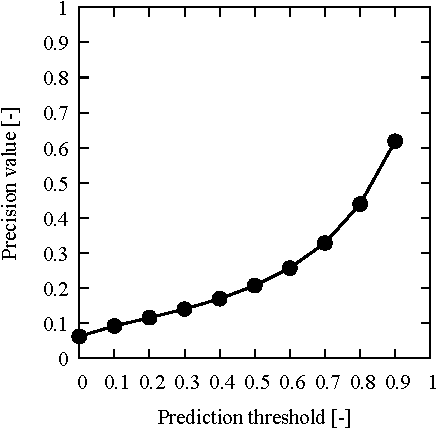
\includegraphics[width=\linewidth]{./Figure/4_Results/training/sresult/precision.pdf}
        \caption{EfficientNetV2-S}
        \label{fig:precisionResult:s}
    \end{subfigure}
    \hfill
    \begin{subfigure}[t]{0.45\linewidth}
        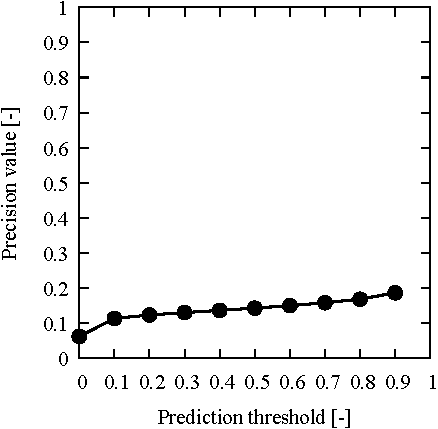
\includegraphics[width=\linewidth]{./Figure/4_Results/training/xlresult/precision.pdf}
        \caption{EfficientNetV2-XL}
        \label{fig:precisionResult:xl}
    \end{subfigure}

    \caption{Precision value for each threshold. The threshold of \num{0.5} is the default value.} 
    \label{fig:precisionResult}
\end{figure}

\begin{figure}[H]
    \centering
    \begin{subfigure}[t]{0.45\linewidth}
        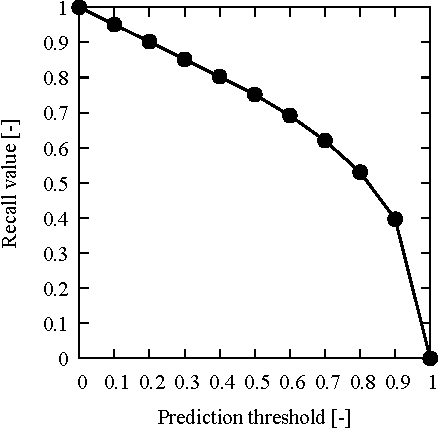
\includegraphics[width=\linewidth]{./Figure/4_Results/training/sresult/recall.pdf}
        \caption{EfficientNetV2-S}
        \label{fig:recallResult:s}
    \end{subfigure}
    \hfill
    \begin{subfigure}[t]{0.45\linewidth}
        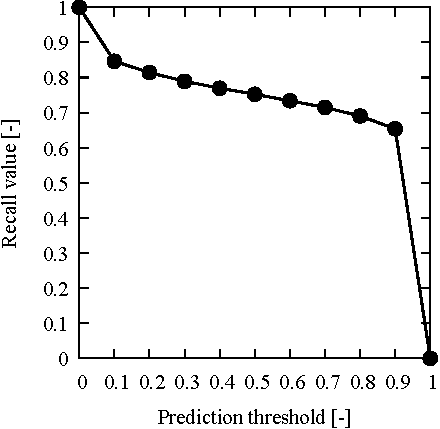
\includegraphics[width=\linewidth]{./Figure/4_Results/training/xlresult/recall.pdf}
        \caption{EfficientNetV2-XL}
        \label{fig:recallResult:xl}
    \end{subfigure}

    \caption{Recall value for each threshold. The threshold of \num{0.5} is the default value.} 
    \label{fig:recallResult}
\end{figure}

\begin{figure}[H]
    \centering
    \begin{subfigure}[t]{0.45\linewidth}
        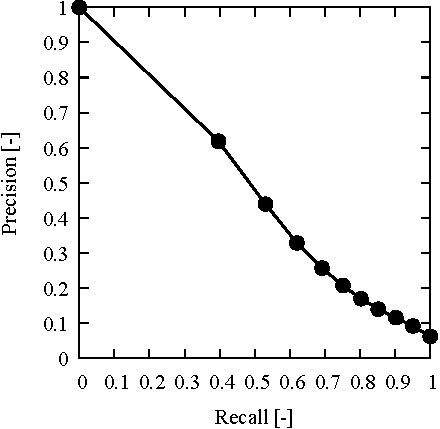
\includegraphics[width=\linewidth]{./Figure/4_Results/training/sresult/prcurve.pdf}
        \caption{Loss improvement of the raw-input model}
        \label{fig:prcurve:s}
    \end{subfigure}
    \hfill
    \begin{subfigure}[t]{0.45\linewidth}
        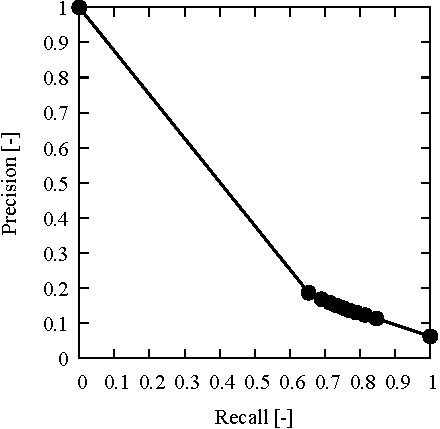
\includegraphics[width=\linewidth]{./Figure/4_Results/training/xlresult/prcurve.pdf}
        \caption{Accuracy improvement of the raw-input model}
        \label{fig:prcurve:xl}
    \end{subfigure}

    \caption{Precision-Recall curve of the raw-input model; each point represents the correspondence between the Recall and Precision values for a given discrimination threshold. Thresholds are taken from 0 to 1 in increments of 0.1.} 
    \label{fig:prcurve}
\end{figure}

\begin{table}[H]
    \centering
    \caption{PR-AUC of the inference result of the trained models. }
    \begin{tabular}{cc}
        Model name & PR-AUC \\ \hline \hline
        EfficientNetV2-S & 0.506 \\ \hline
        EfficientNetV2-XL & 0.571 \\
    \end{tabular}
    \label{table:prauc}
\end{table}

\subsection{衝突水滴組の軌跡再生}
本節では,実験で記録した衝突水滴ホログラムに対する推論のデモンストレーションを行う.\ref{sec:modelEvalResult}節で示した通り,モデルは十分な衝突水滴検出性能を有しているとは言えず,そのため実験データから水滴衝突に関わる統計的な情報を正しく得ることはできない.しかし,実際に構築したモデルを用いて実験データに対する推論を行い,その結果を可視化する手法を整備することは今後の研究のために有用である.したがって,実験データに対するEfficientNetV2-XLモデルによる推論結果を位相回復ホログラフィによる3次元像再生によって確認する.Fig. \ref{fig:expInfResult}に実験データに対する推論の可視化結果の例を示す.この例では,濃い赤色で示す領域で\num{1.00}の確率で水滴近接が推定されている.このホログラムを観測体積で再生し,$x$-$y$軸の投影像を二値化して得られる画像をFig. \ref{fig:expHoloImp}に示す.二値化のためのしきい値決定にはMinimum法\cite{prewitt1966}を用いた.高い近接確率を示した領域で水滴が近接していることがわかる.

次に,Fig. \ref{fig:expHoloImp}に示した投影像から粒子検出を行いその$x$,$y$座標と水滴径を決定する.これらの情報と,\ref{sec:particleDepth}節に示した奥行位置決定手法を用いて,観測体積内の3次元水滴分布を決定する.その結果をFig. \ref{fig:3dview}に示す.また,この抽出フレーム前後の水滴軌跡を可視化した3次元分布をFig. \ref{fig:3dtrajectory}に示す.この例では,波線で示した矩形領域で水滴併合が発生している.$x$-$y$投影図において,2つの水滴が近接・併合しその後水滴半径が増加していることがわかる.しかし,Tamuraの方法ではこの例のように水滴数密度が大きいときに水滴の高精度な奥行位置決定が困難であり,推定された奥行方向位置の誤差が大きく軌跡がなめらかに接続していない.そのため,$z$軸を含むプロットから併合水滴を目視で確認するのは困難である.したがって,併合水滴組のみの軌跡をFig. \ref{fig:3dtrajectory_detail}に,そのうち$x$-$z$投影図の累積軌跡を示す.ここでの累積軌跡は,はじめのフレームからあるフレームまでの水滴軌跡を重畳した軌跡プロットである.これらの図から,$z$軸正方向・負方向にそれぞれ運動している2つの水滴が近接し併合していることがわかる.

これらの結果から,EfficientNetV2-XLモデルによる推論結果を用いて,実験データから併合水滴の軌跡を抽出できることがわかる.今後,多くの水滴衝突・併合を抽出し衝突・併合に関する統計量を正確に算出するには,水滴近接検出よりも正確な併合判定システムが必要であり,そのためにTamuraの方法による奥行位置決定手法の改善が重要である.




\begin{figure}[H]
    \centering
    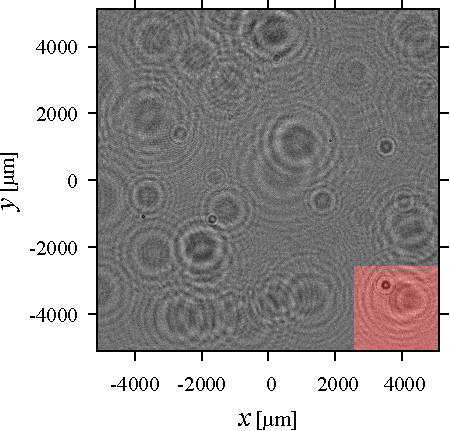
\includegraphics[width=0.8\linewidth]{./Figure/4_Results/exp/visout.pdf}
    \caption{Example of the inference result of the raw-input model, for the experimentally recorded hologram. The confidence value on the red shade area of the top right corner is \num{1.00}. This output image is contrast-enhanced for visualization.}
    \label{fig:expInfResult}
\end{figure}

\begin{figure}[H]
    \centering
    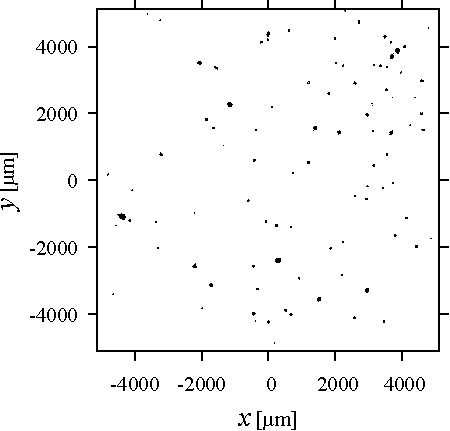
\includegraphics[width=0.8\linewidth]{./Figure/4_Results/exp/imp.pdf}
    \caption{$x$-$y$ projection of the reconstructed volume shown in Fig. \ref{fig:expInfResult}}
    \label{fig:expHoloImp}
\end{figure}

\begin{figure}[H]
    \centering
    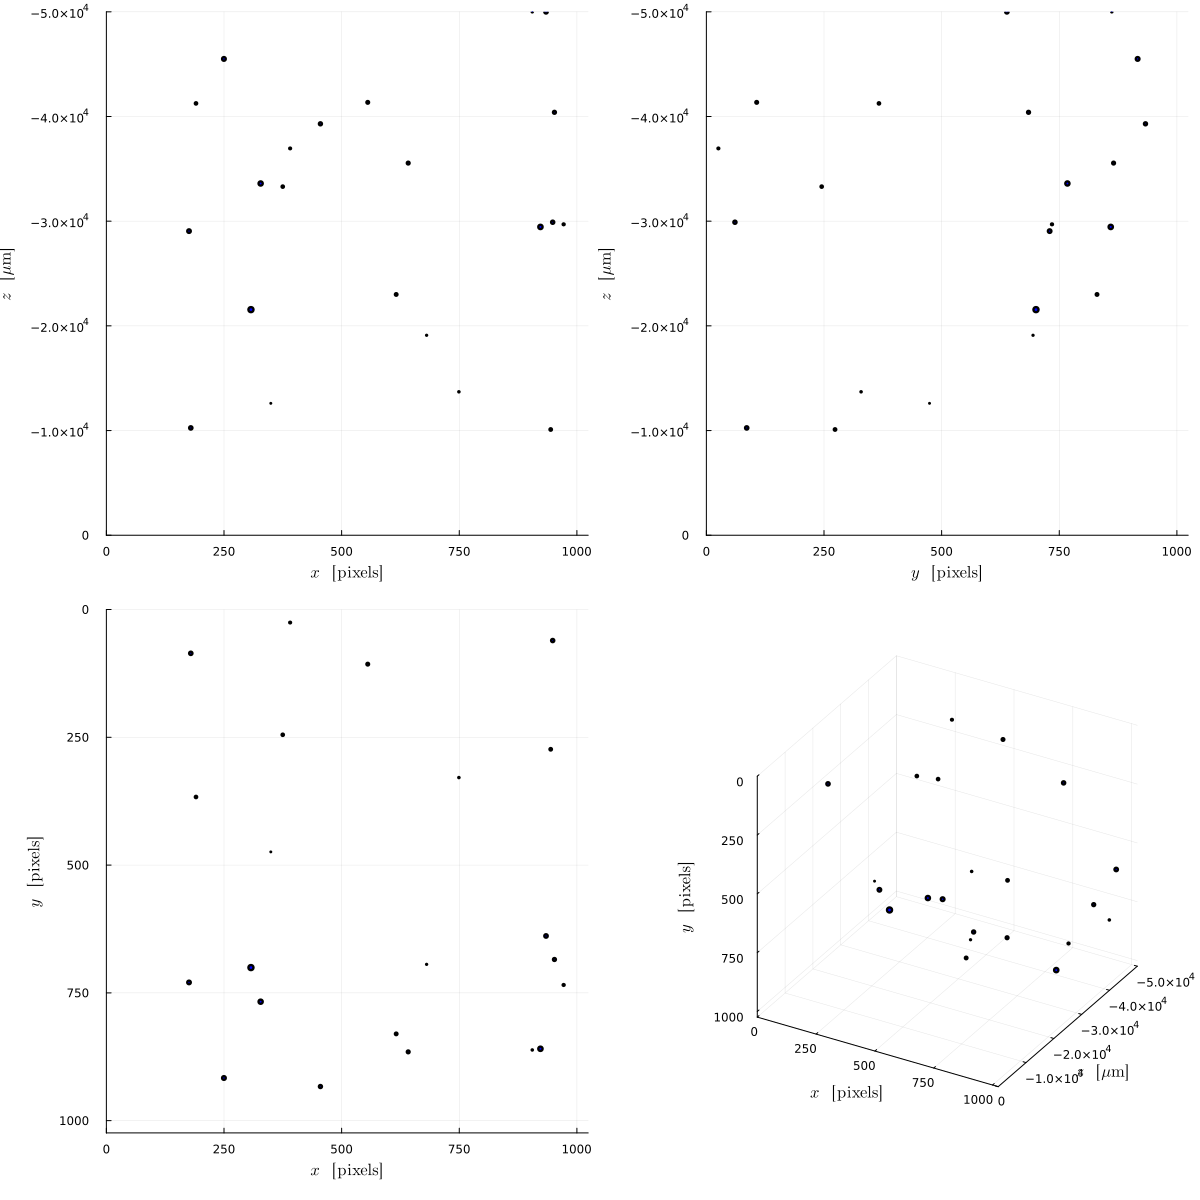
\includegraphics[width=0.98\linewidth]{./Figure/4_Results/exp/3dview.png}
    \caption{Three dimensional view of the reconstructed volume shown in Fig. \ref{fig:expInfResult}. There is an approaching droplet pair in the red shaded area shown in Fig. \ref{fig:expInfResult}.}
    \label{fig:3dview}
\end{figure}

\begin{figure}[H]
    \centering
    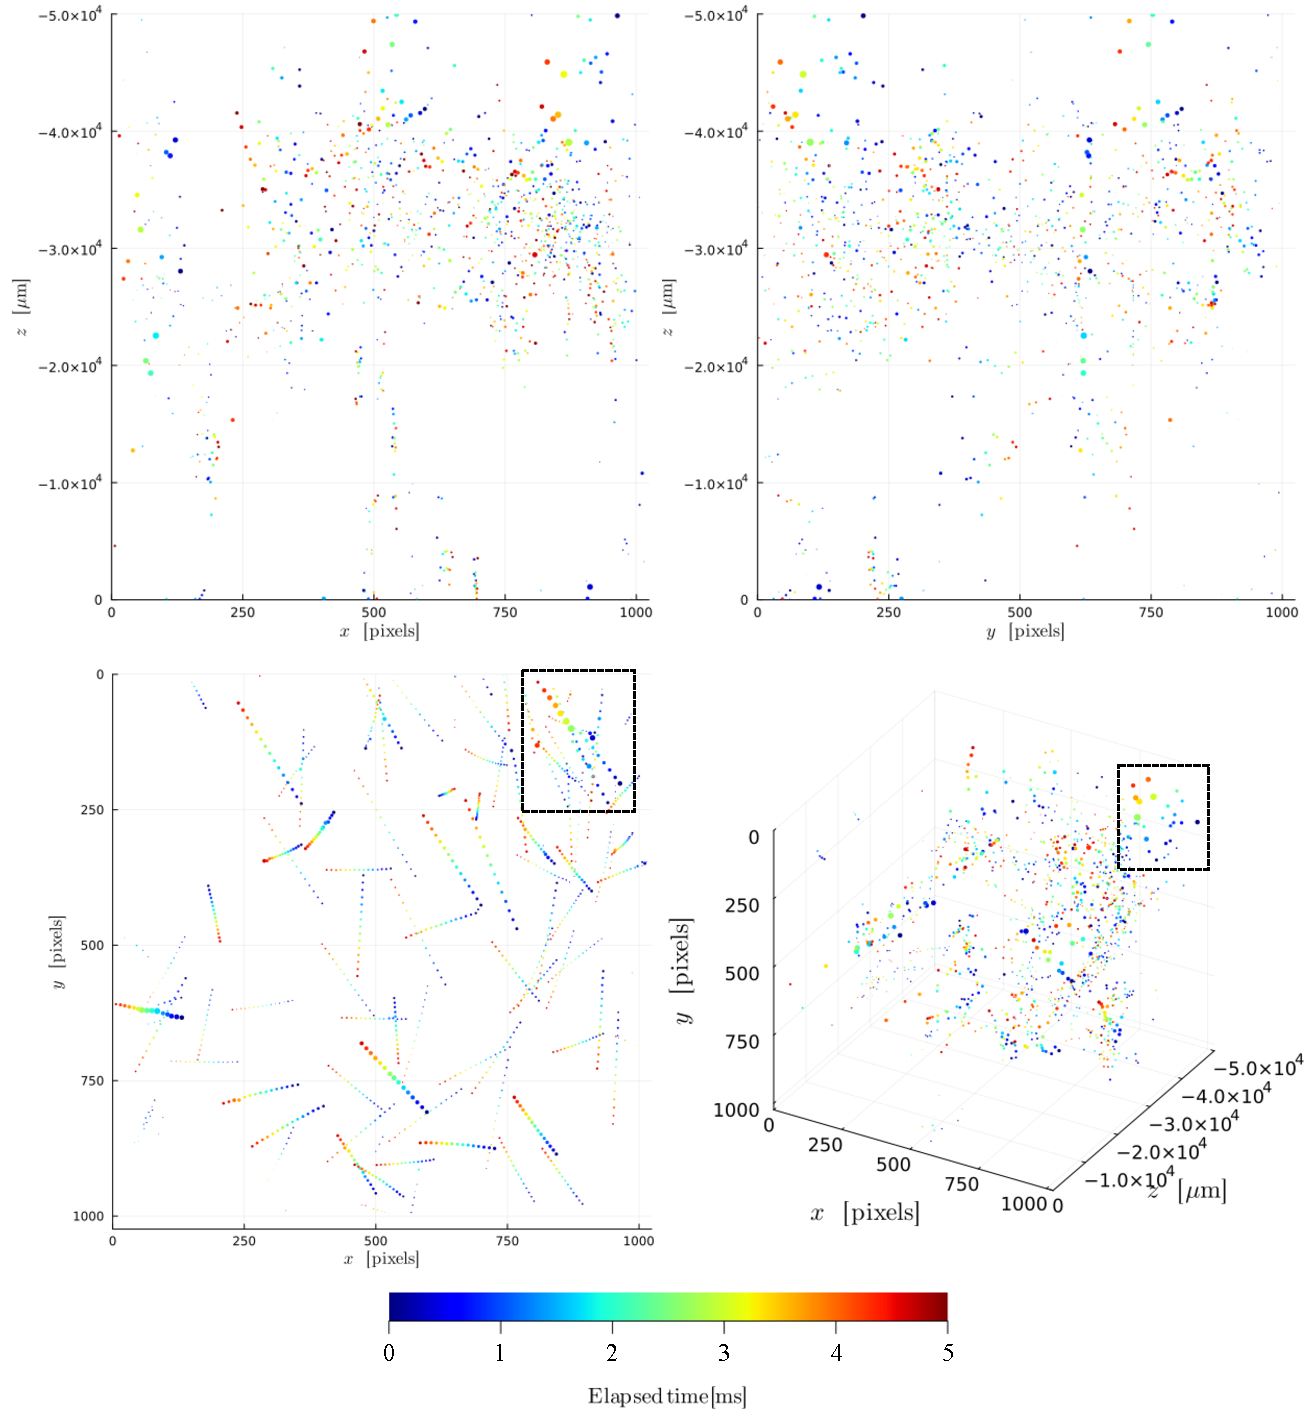
\includegraphics[width=1.00\linewidth]{./Figure/4_Results/exp/3dtraj.pdf}
    \caption{Reconstructed droplet trajectories; the droplet marker color changes from blue to red as time progresses. Droplet diameter corresponds to the marker size. Two droplets coalesce in the upper right corner of the x-y plane, indicated by the dashed rectangular area, and the droplet diameter increases.}
    \label{fig:3dtrajectory}
\end{figure}

\begin{figure}[H]
    \centering
    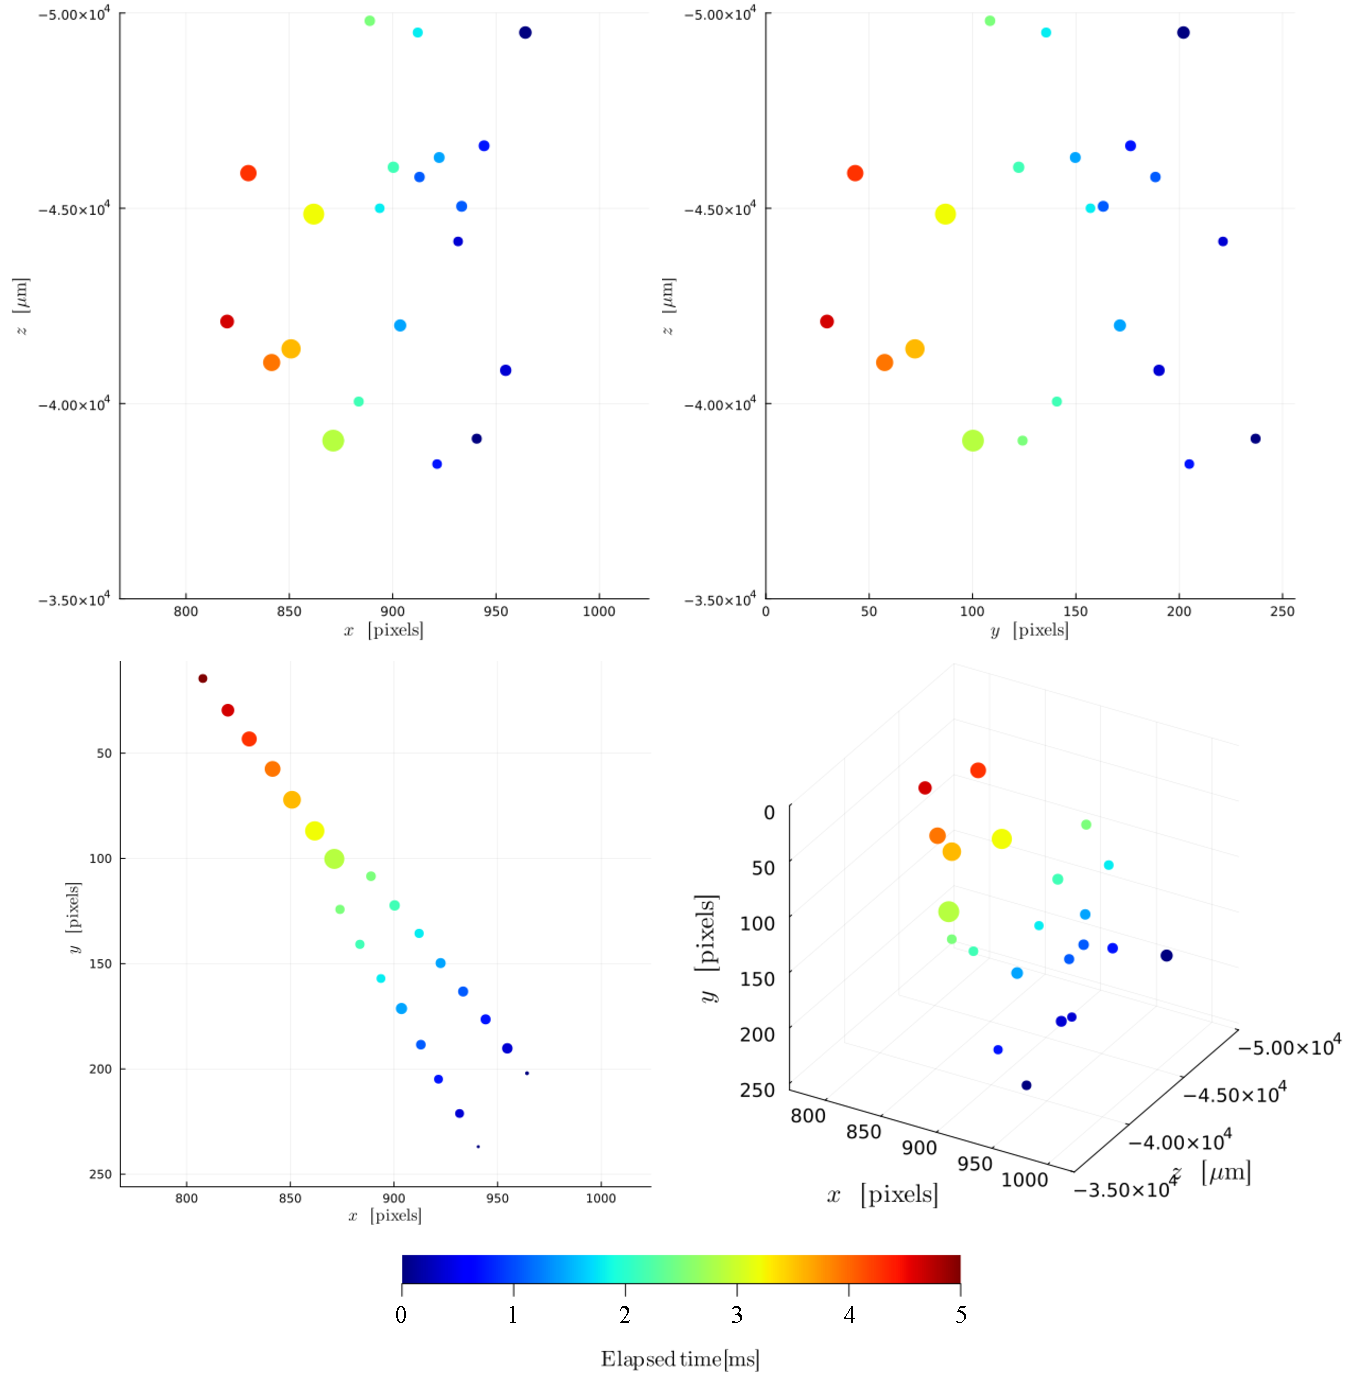
\includegraphics[width=1.00\linewidth]{./Figure/4_Results/exp/traj_detail.pdf}
    \caption{Trajectory plots obtained by reconstructing only the coalesced droplet pairs. Trajectory shape is unclear due to large variance in depth position estimation by the Tamura's method.}
    \label{fig:3dtrajectory_detail}
\end{figure}

\begin{figure}[H]
    \centering
    \begin{subfigure}[t]{0.32\linewidth}
        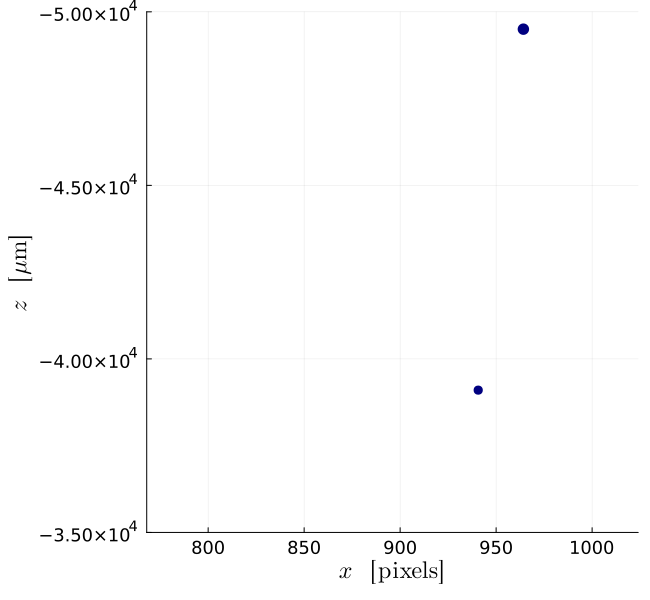
\includegraphics[width=\linewidth]{./Figure/4_Results/exp/xz_detailed_view/out0001.png}
        \caption*{$t = \SI{0}{\ms}$}
    \end{subfigure}
    \begin{subfigure}[t]{0.32\linewidth}
        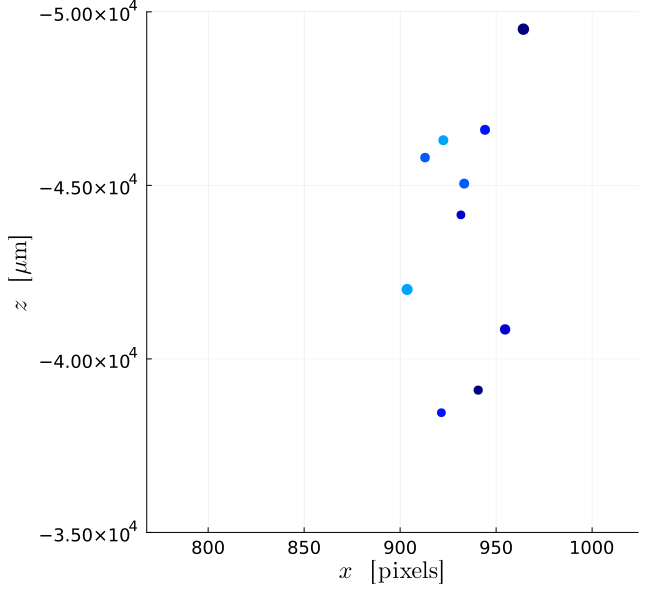
\includegraphics[width=\linewidth]{./Figure/4_Results/exp/xz_detailed_view/out0005.png}
        \caption*{$t = \SI{1.0}{\ms}$}
    \end{subfigure}
    \\
    \begin{subfigure}[t]{0.32\linewidth}
        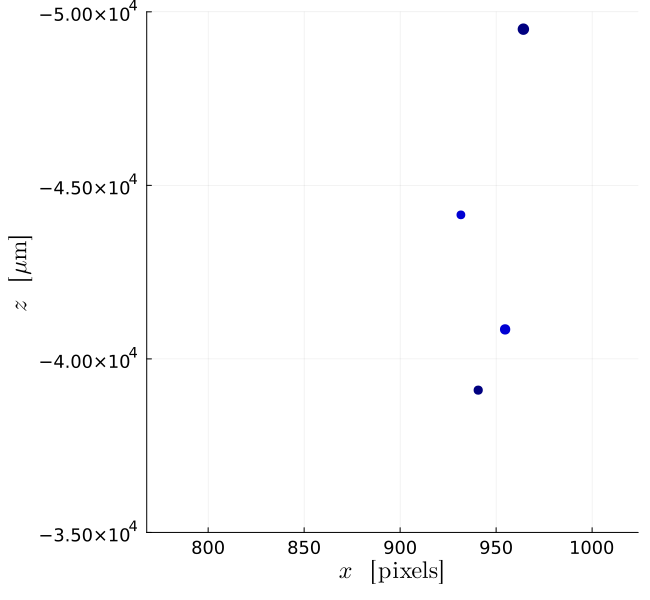
\includegraphics[width=\linewidth]{./Figure/4_Results/exp/xz_detailed_view/out0002.png}
        \caption*{$t = \SI{0.25}{\ms}$}
    \end{subfigure}
    \begin{subfigure}[t]{0.32\linewidth}
        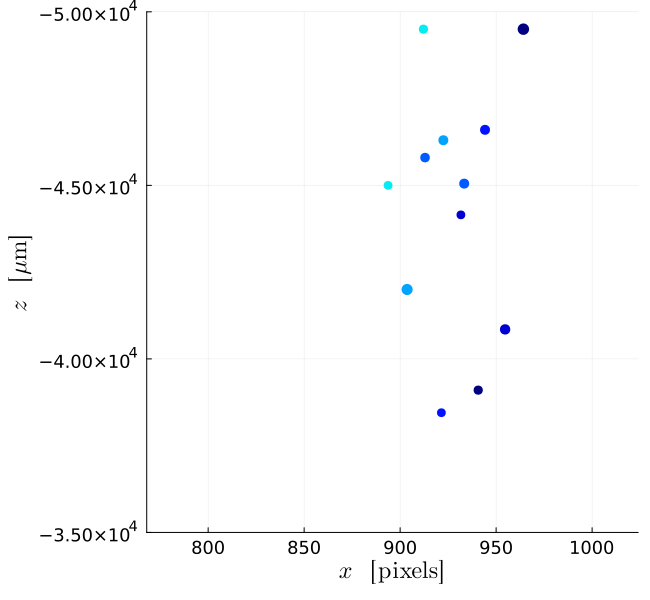
\includegraphics[width=\linewidth]{./Figure/4_Results/exp/xz_detailed_view/out0006.png}
        \caption*{$t = \SI{1.25}{\ms}$}
    \end{subfigure}
    \\
    \begin{subfigure}[t]{0.32\linewidth}
        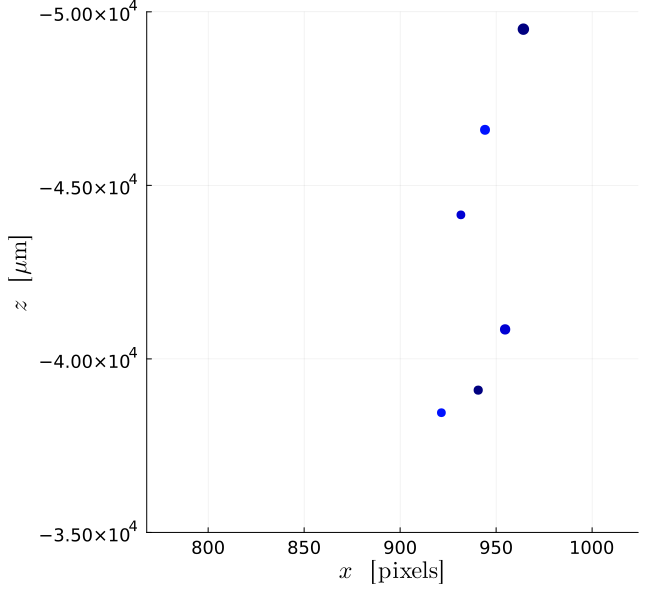
\includegraphics[width=\linewidth]{./Figure/4_Results/exp/xz_detailed_view/out0003.png}
        \caption*{$t = \SI{0.5}{\ms}$}
    \end{subfigure}
    \begin{subfigure}[t]{0.32\linewidth}
        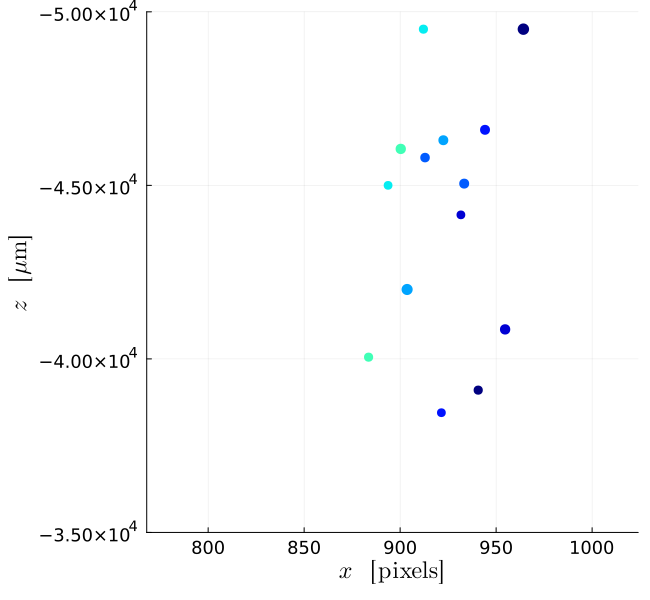
\includegraphics[width=\linewidth]{./Figure/4_Results/exp/xz_detailed_view/out0007.png}
        \caption*{$t = \SI{1.5}{\ms}$}
    \end{subfigure}
    \\
    \begin{subfigure}[t]{0.32\linewidth}
        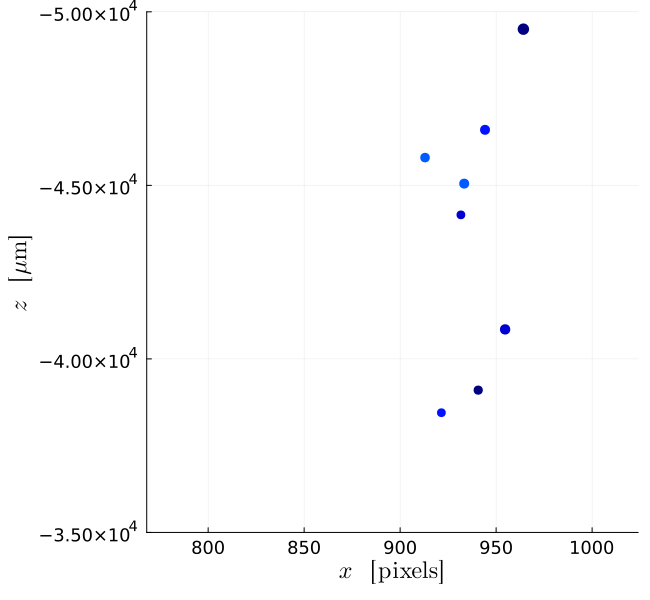
\includegraphics[width=\linewidth]{./Figure/4_Results/exp/xz_detailed_view/out0004.png}
        \caption*{$t = \SI{0.75}{\ms}$}
    \end{subfigure}
    \begin{subfigure}[t]{0.32\linewidth}
        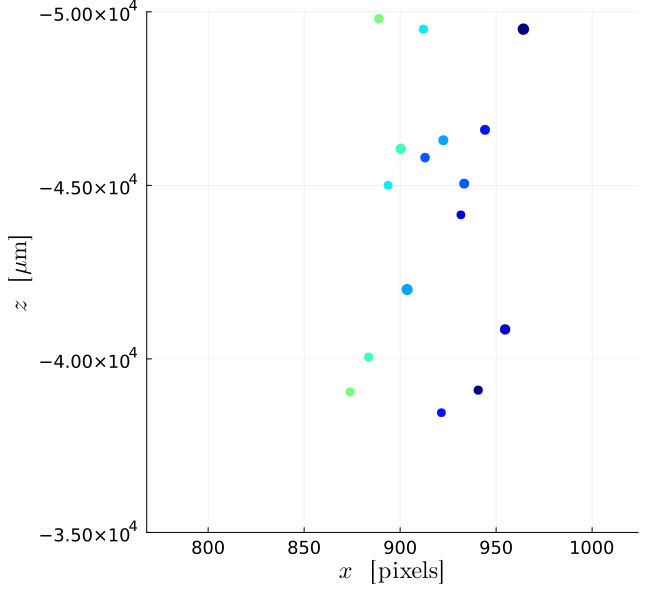
\includegraphics[width=\linewidth]{./Figure/4_Results/exp/xz_detailed_view/out0008.png}
        \caption*{$t = \SI{1.75}{\ms}$}
    \end{subfigure}

    \caption{Detail of $x$-$z$ projection of coalesced droplets.}
    \label{fig:xz_detailed_view}
\end{figure}

\begin{figure}[H]
    \addtocounter{figure}{-1}
    \centering
    \begin{subfigure}[t]{0.32\linewidth}
        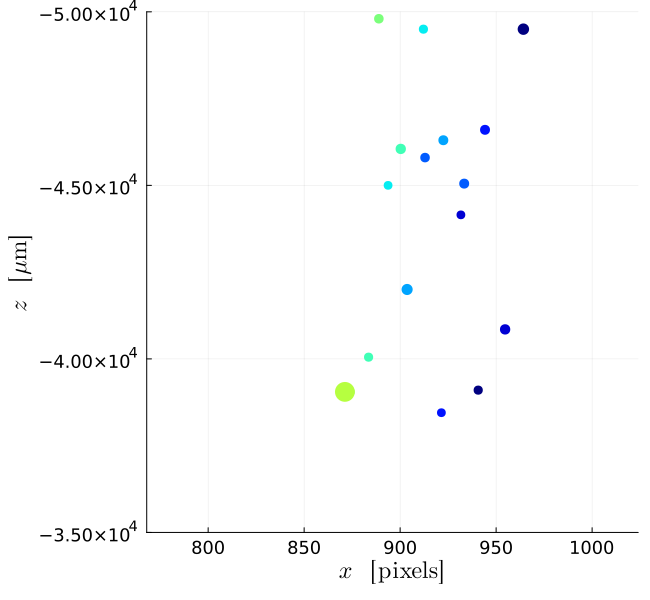
\includegraphics[width=\linewidth]{./Figure/4_Results/exp/xz_detailed_view/out0009.png}
        \caption*{$t = \SI{2.0}{\ms}$}
    \end{subfigure}
    \begin{subfigure}[t]{0.32\linewidth}
        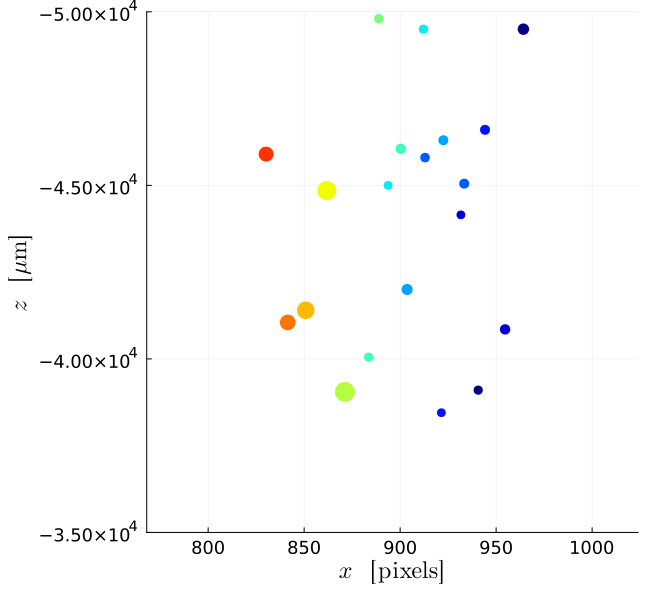
\includegraphics[width=\linewidth]{./Figure/4_Results/exp/xz_detailed_view/out0013.png}
        \caption*{$t = \SI{3.0}{\ms}$}
    \end{subfigure}
    \\
    \begin{subfigure}[t]{0.32\linewidth}
        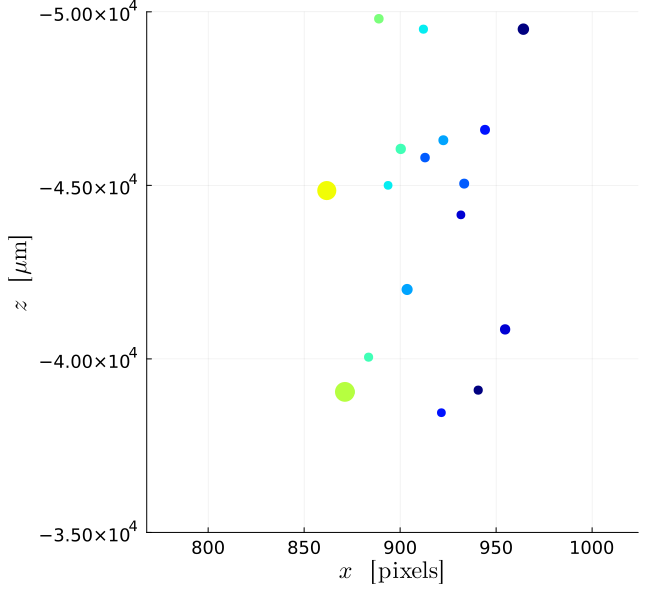
\includegraphics[width=\linewidth]{./Figure/4_Results/exp/xz_detailed_view/out0010.png}
        \caption*{$t = \SI{2.25}{\ms}$}
    \end{subfigure}
    \begin{subfigure}[t]{0.32\linewidth}
        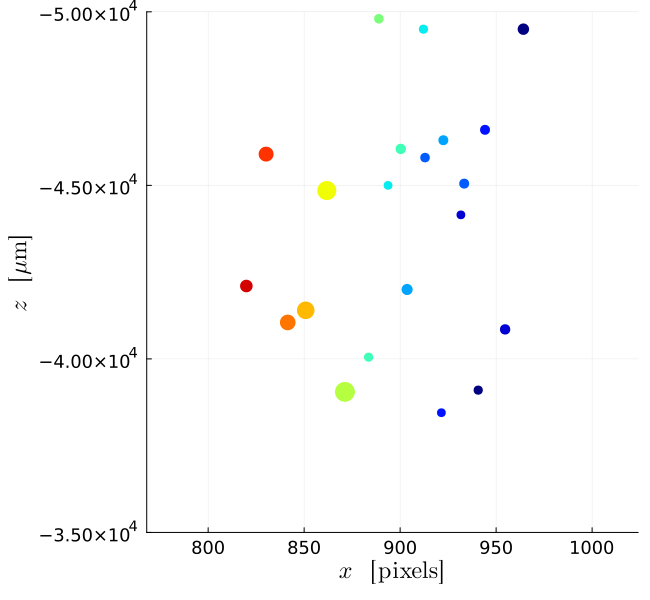
\includegraphics[width=\linewidth]{./Figure/4_Results/exp/xz_detailed_view/out0014.png}
        \caption*{$t = \SI{3.25}{\ms}$}
    \end{subfigure}
    \\
    \begin{subfigure}[t]{0.32\linewidth}
        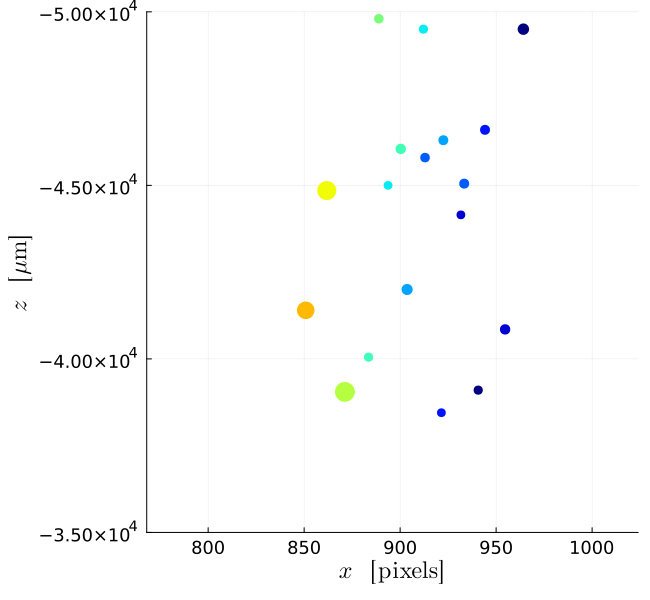
\includegraphics[width=\linewidth]{./Figure/4_Results/exp/xz_detailed_view/out0011.png}
        \caption*{$t = \SI{2.5}{\ms}$}
    \end{subfigure}
    \begin{subfigure}[t]{0.32\linewidth}
        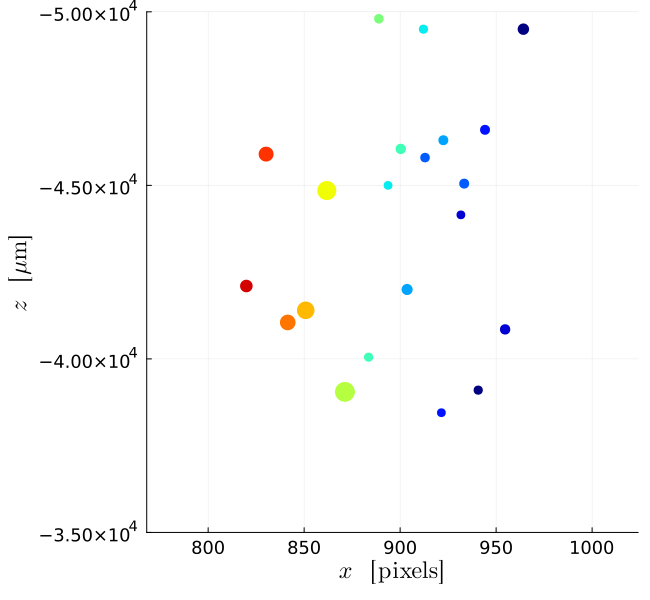
\includegraphics[width=\linewidth]{./Figure/4_Results/exp/xz_detailed_view/out0015.png}
        \caption*{$t = \SI{3.5}{m\s}$}
    \end{subfigure}
    \\
    \begin{subfigure}[t]{0.32\linewidth}
        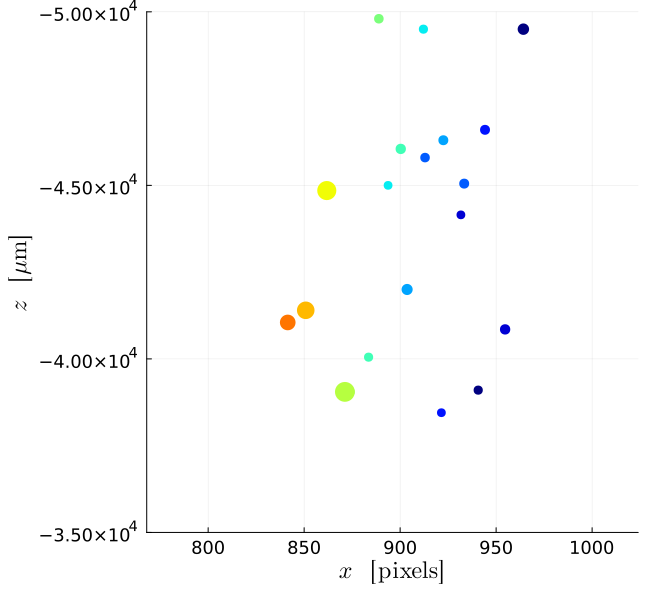
\includegraphics[width=\linewidth]{./Figure/4_Results/exp/xz_detailed_view/out0012.png}
        \caption*{$t = \SI{2.75}{\ms}$}
    \end{subfigure}
    \hspace{0.32\linewidth}
    \caption{Detail of $x$-$z$ projection of coalesced droplets.}
\end{figure}
